\section{Aplikacja główna}


{\color{red}tutaj będą makiety}

\subsection{Świat gry}

\begin{center}
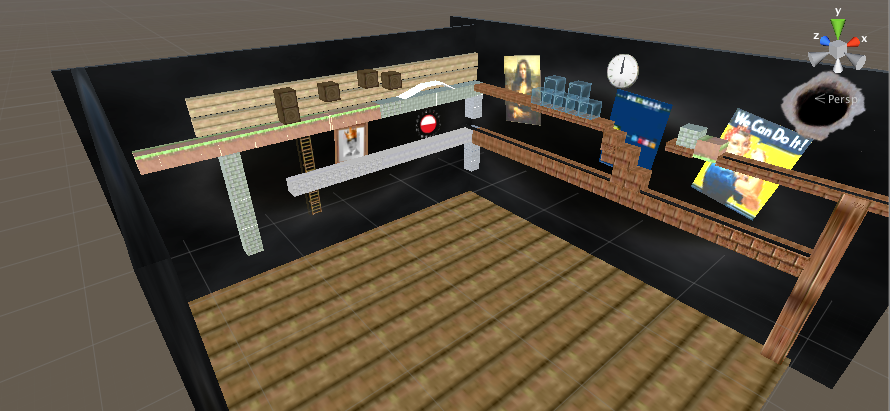
\includegraphics[width=0.9\textwidth]{images/swiatgry.png}
\captionof{figure}{
Model w środowisku Unity
}
\small {źródło: własne }
\end{center}


\subsection{Aktorzy}

\begin{center}

 \begin{tabular}{|c|c|}
 \hline  
  &   \\
  \hline   
  &   \\
  \hline   
\end{tabular}
\captionof{table}{Właściwości aktora}
\end{center}

\begin{lstlisting}[language=CSharp]
public void SendInfo() {
	Network.SendMessage("hasax_"+this.hasAx);
	Network.SendMessage("hassh_"+this.hasSh);
	Network.SendMessage("hasdrabina_"+this.drabina);
	Network.SendMessage("isMove_"+this.isMove);
}
\end{lstlisting}
\captionof{lstlisting}{
	Do Poprawy
}

\subsection{Kamery}
\paragraph{}
Platforma Unity wspiera do 8 wirtualnych kamer \footnote{http://docs.unity3d.com/Manual/MultiDisplay.html}.
Każda z tych kamer może być prezentowana na oddzielnym fizycznym ekranie.

\subsection{Prefabrykaty}
\paragraph{}
W Unity możliwe jest używanie prefabrykatów (Prefabs \footnote{http://docs.unity3d.com/Manual/Prefabs.html}). Są obiekty lub grupy obiektów, które służą do wielokrotnego wykorzystywania. W Projekcie założono, że wszystkie reużwalne komponety (dziedziczone pomiędzy scenami) będą prefabrykatami.

Dodatkowo aktorzy gry (generowane dynamicznie) są również prefabrykatami. Instancje aktora są tworzone podczas działania aplikacji.

{\color{red}Opisać prefabrykaty}

\subsection{Logika biznesowa}
\subsection{Serwer komunikacyjny}